\documentclass[uct_visualisation_thesis.tex]{subfiles}

\section{Algorytmy MCTS}
\subsection{Opis grupy algorytmów} \label{subsec:mcts_group}
Monte-Carlo Tree Search to heurystyka, której celem jest podejmowanie decyzji w pewnych zadaniach sztucznej inteligencji, na przykład wybieranie ruchów w grach. Metoda jest oparta na przeszukiwaniu możliwych stanów gry zapisanych w wierzchołkach drzewa i losowym symulowaniu rozgrywek. Algorytmy MCTS opierają się na rozbudowywaniu drzewa ze stanami gry poprzez iteracyjne wykonywanie czterech faz. Jednym z najpowszechniejszych wariantów MCTS jest algorytm UCT. Pseudokod opisany w listingu \ref{lst:mcts} oraz implementacja MCTS w projekcie bazują na \cite{banditbased}. Przykład działania algorytmu ze szczególnym uwzględnieniem kolejnych faz znajduje się na rysunku \ref{rys:mcts_phases}.
\begin{figure}[h]
	\centering
	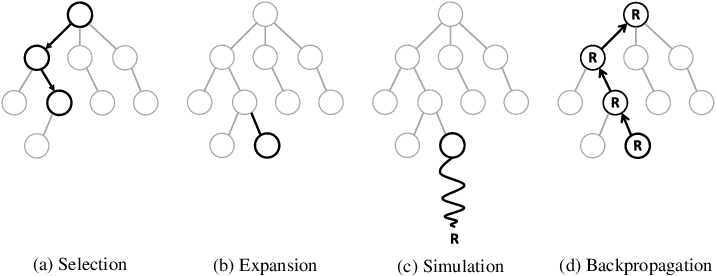
\includegraphics[width=0.8\textwidth]{mcts_phases.png}
	\caption{Fazy MCTS}
	\label{rys:mcts_phases}
\end{figure}

\begin{enumerate}
	\item \textbf{Faza wyboru} (linia 7 w listingu) -- wybór najbardziej obiecującego wierzchołka do rozrostu drzewa. Istotny w tej fazie jest balans pomiędzy eksploatacją ruchów przeanalizowanych najdokładniej oraz eksploracją tych jeszcze niezbadanych. Przez eksploatację wierzchołka powinno rozumieć się powiększanie rozmiaru drzewa tworzonego przez nie, a przez eksplorację --- rozwijanie wierzchołków, które uprzednio nie miały żadnych potomków.
	\item \textbf{Faza rozrostu} (linia 9 w listingu) -- utworzenie wierzchołków potomnych dla najbardziej obiecującego wierzchołka drzewa. Tworzone wierzchołki odpowiadają stanom możliwym do uzyskania poprzez wykonanie jednego ruchu ze stanu wierzchołka obiecującego.
	\item \textbf{Faza symulacji} (linia 11 w listingu) -- rozegranie partii składającej się z losowych ruchów ze stanu jednego z wierzchołków utworzonych w poprzedniej fazie. Rozgrywana jest ona do końca, czyli do wyłonienia zwycięzcy lub spowodowania remisu, lub jest ucinana po pewnej liczbie ustalonych ruchów i wynik gry jest ewaluowany przez pewną funkcję.
	\item \textbf{Faza propagacji wstecznej} (linia 13 w listingu) -- aktualizacja informacji na temat wierzchołków na ścieżce od wierzchołka-liścia, z którego rozpoczęto symulację, do korzenia drzewa. Główną przekazywaną wartością jest wynik symulacji.
\end{enumerate}

\begin{minipage}{\linewidth} % minipage to ensure listing is on seperate page
\begin{lstlisting}[caption={Pseudokod algorytmu Monte Carlo Tree Search}, label=lst:mcts, style=mystyle]
def find_next_move(curr_state):
	iterations_counter = 0
	tree = initialize_tree(curr_state)
	
	while iterations_counter < max_iterations_counter:
		# selection(tree.root) 
		curr_node = select promising node    
		# expansion(node)
		create child nodes from node
		# simulation(node)		
		playout_result = simulate random playout from curr_node     
		# backpropagation(node, playout_result)
		update tree according to playout_result                     
		
		iterations_counter++
	
	best_state = select best child(tree.root) 
	return best_state
\end{lstlisting}
\end{minipage}


\section{Algorytm UCT}
\subsection{Opis algorytmu} \label{subsec:uct}
UCT jest wariantem metody MCTS, który stara się zachować równowagę między eksploatacją ruchów o wysokiej średniej wygranej a eksploracją tych mało zbadanych. Formuła, która odpowiada za wyznaczenie najbardziej obiecującego wierzchołka w fazie wyboru MCTS jest przedstawiona jako wyrażenie \ref{formula:uct}.

\begin{equation}\label{formula:uct}
\frac{w_i}{n_i} + c \sqrt{\frac{\ln N_i}{n_i}}
\end{equation}

W wyrażeniu \ref{formula:uct}, indeks $i$ odnosi się do liczby wykonanych przez algorytm iteracji, czyli czterech faz MCTS. W pierwszym składniku sumy wyrażenia \ref{formula:uct}, licznik $w_i$ oznacza liczbę wygranych w danym węźle, a mianownik $n_i$ oznacza liczbę rozegranych symulacji. Zatem ułamek ten przyjmuje wartości większe dla ruchów o większej średniej wygranej, co odpowiada ze eksploatację drzewa. Drugi składnik sumy wyrażenia \ref{formula:uct} przyjmuje wartości większe dla wierzchołków, dla których wykonano mniej symulacji i odpowiada eksploracji drzewa. $N_i=\sum_i n_i$, a
$c$ jest parametrem eksploracji, który może być dostosowany do badanego problemu (najczęściej przyjmuje się $c=\sqrt{2}$).


\subsection{Dodatkowe założenia}
Stworzone przez nas rozwiązanie dodaje pewne założenia do algorytmu UCT. Dodanie założeń pozwoliło nam na stworzenie rozwiązania bardziej uniwersalnego i niezależnego od zasad i logiki badanych gier. 

\begin{enumerate}
	\item Rozgrywka jest prowadzona naprzemiennie przez dwóch graczy.
	\item Każdy ruch ma jednoznaczny wpływ na dalszą rozgrywkę (rozgrywka jest deterministyczna).
	\item Każdy z graczy ma dostęp do pełnej informacji o aktualnym stanie gry.
\end{enumerate}


\section{Algorytm wizualizacji drzewa}

\subsection{Określenie problematyki}
Celem prezentowanego rozwiązania jest wizualizacja drzewa w sposób najbardziej przejrzysty dla użytkownika. Ma to ułatwić użytkownikowi poznanie struktury drzewa i zależności między wierzchołkami. Jako że zaprojektowanie układu wierzchołków przy pewnych założeniach jest problemem NP-zupełnym nawet dla drzew binarnych, co zostało opisane w \cite{treelayout}, w prezentowanym rozwiązaniu posłużymy się heurystyką.

\subsection{Założenia}
W celu uczynienia wizualizacji jak najbardziej czytelną, poczyniliśmy pewne założenia w kontekście układu wierzchołków i krawędzi wizualizowanych drzew. Zostały one wymienione poniżej. 

\begin{enumerate}
	\item Krawędzie drzewa nie mogą się przecinać.
	\item Wierzchołki będą ustawione od góry w rzędach, a przynależność do
	rzędów będzie zależała od odległości wierzchołków od korzenia.
	\item Wierzchołki mają być narysowane możliwie najwęziej.
\end{enumerate}


\subsection{Usprawniony algorytm Walkera}
W celu wyznaczenia układ wierzchołków drzewa na płaszczyźnie, spełniając powyższe 3 założenia, skorzystamy z usprawnionego algorytmu Walkera, który działa w czasie liniowym względem liczby wierzchołków. Algorytm, który zaimplementowaliśmy, został opisany w \cite{impwalkers}.